%================================================================
\chapter{Introduction and Objective of the Study}
%================================================================

%================================================================
\section{Introduction}\label{sec:Introduction}
%================================================================

%================================================================
\subsection{Machine Learning}\label{sec:Machine Learning Intro}
%================================================================


\emph{Machine learning} is a highly field of study involving algorithms that allow computers to solve problems using data, relieving the need for tailoring problem-specific solutions \cite{SupervisedwquantumComputers}. This practice has transformed nearly every aspect of our modern society, from medicine \cite{medicine} to finance \cite{finance}. One branch of machine learning is \emph{supervised learning}, which is the practice of training a model to learn a relation between input and output data \cite{hastie01statisticallearning}. Typically, one starts by acquiring a \emph{training set} of \emph{labelled data}, which is a collection of pairs of input and output data. As an example, the inputs and outputs can be \emph{age} and \emph{salary} of people, respectively. By training a machine learning model on the training set, the aim is that it "learns" the general relation between \emph{age} and \emph{salary}. If this is the case, the model can be used ti predict the salary of people based on their age, even for values of \emph{age} not present in the training set. If the latter is the case, the model is said to generalize to unseen data, which is required for prediction. How are machine learning models trained? It is typical to define a \emph{loss function} (also commonly known as risk, cost or error function \citet{}), which is a scalar function that measures how accurately a model predicts the outputs from the corresponding inputs \cite{hastie01statisticallearning}. The lower the value of the loss function, the better the model reproduces the outputs. Therefore, training a model involves minimizing the loss function with respect to the training set.

A particular powerful family of machine learning models are the \emph{neural networks} (NN). Neural networks are models consisting of layers of artificial neurons, originally inspired by the neural structures in the brain \cite{hands-on}. They are \emph{parametric} models, meaning that the input-output relation that they compute are determined by a set of real-valued parameters. When setting up a NN, the goal of the training is to find the correct parameters such that the given loss function is minimized. This is done by calculating the derivative of the loss function with respect to the parameters of the NN. This derivative is called the \emph{gradient}, which quantifies how the loss function changes when the parameters are adjusted. Using gradient-based methods, such as gradient descent, the gradient can be utilized to adjust the parameters such that the loss decreases \cite{hands-on}. The \emph{backpropagation algorithm}, tailored for accommodating their layered structure, is commonly used for calculating the gradient of NNs \cite{hands-on}. 

Increasing the number of layers of NNs has been shown to increase their flexibility \cite{raghu2017expressive}, meaning that they can reproduce the input-output pairs of complex data more easily. However, this comes with a drawback: with increasing number of layers, the \emph{vanishing gradient phenomenon} emerges, meaning the magnitude of the gradient decreases exponentially \cite{LeCun2012}. This phenomenon manifests itself as a loss function that is insensitive to adjustments of the parameters, known as a flat \emph{loss landscape}, making the training of many-layered NNs difficult \cite{karakida2019universal}. To uncover the geometry of the loss landscape, and determine its flatness, it is common practice to assess the spectrum of the \emph{empirical fisher information matrix} (EFIM) \cite{karakida2019universal}.


%================================================================
\subsection{Quantum Computing}\label{sec:Quantum Computing Intro}
%================================================================
\emph{Quantum computing} is the processing of information using systems that obey the laws of quantum mechanics \cite{NielsenQuantum}. In 1982, Richard Feynman pointed out that quantum mechanical systems are notoriously difficult to simulate on classical computers. He suggested that this complexity c b be exploited by build a computer based on the principals of quantum mechanics \cite{NielsenQuantum}. Only three years later, David Deutsch formalized a theory describing such a device, a \emph{universal quantum computer} \cite{Deutsch1985QuantumTT}. Even though such a device was not yet realized physically, people started developing algorithms for quantum computers that theorized to be more efficient than their classical counterparts. In 1996, physicist Seth Lloyd showed that quantum mechanical systems could be efficiently simulated on quantum computers \cite{Lloyd1073}. This is perhaps a result not too surprising, since quantum mechanics is the "native language" of quantum computers. A more surprising discovery happened two years prior, when Peter Shor developed Shor's algorithm for prime factorization of integers in polynomial time, a type of problem which does not spring naturally from the realm of quantum mechanics. Prime factorization is believed to be exponentially hard on classical computers, and the effectiveness of Shor's algorithm shows that the capabilities of quantum computers go beyond the simulation of quantum mechanical systems \cite{Shor_1997}.
This has sparked a huge interest in mapping out what type of problems quantum computing can excel at. 


Today, there is a lot of focus on making quantum computers, with big companies such as Google and IBM at the forefront. Despite the effort, today's quantum computers are not able to implement useful quantum algorithms that would change the world right away. This is because today's quantum computers are small and perform very noisy computations \cite{Preskill_2018}. As it performs an algorithm, also called a \emph{circuit}, it manipulates a very delicate quantum state. During the span of the computation, the state is susceptible to interference from the surrounding environment, causing the information of the system to degrade. This phenomenon is called \emph{decoherence}, and puts a strict limit on length of the circuit one can implement \cite{saki2019study}. This makes many of the more promising quantum algorithms, such as Shor's algorithm, unfeasible to implement today.


%================================================================
\subsection{Quantum Machine Learning}\label{sec:Quantum Machine Learning}
%================================================================
Could quantum computing be useful for developing algorithms for machine learning? By combining machine learning and quantum computing, you get the emerging interdisciplinary field \emph{quantum machine learning}. Just from the name, it is not immediately what it might entail, and as matter of fact, it depends on the context. From \autoref{fig:cccq}, we see the different ways machine learning and quantum computing can be combining. The CC case refers to classical data that is processed on classical devices, which is of course the traditional form of machine learning, e.g. neural networks. The other case, CQ, investigates how classical data can be processed with help of quantum computers. These are the two cases we will focus on in this thesis.

\begin{figure}[htp]
    \centering
    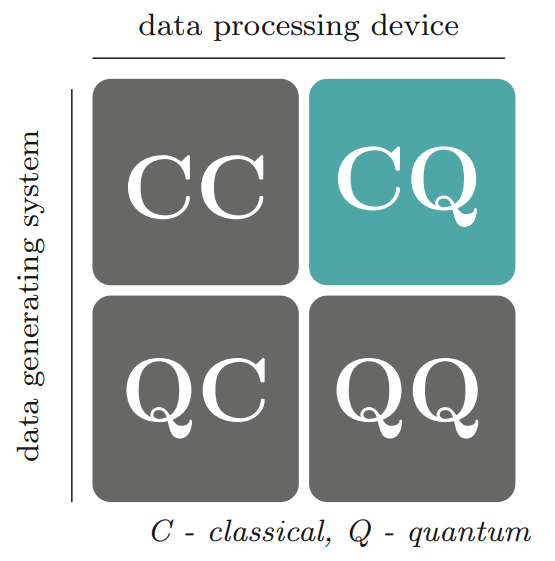
\includegraphics[width=8cm]{latex/figures/cccq.PNG}
    \caption{Four approaches that combine machine learning and quantum computing. The figure is retrieved from \citet{SupervisedwquantumComputers}.}
    \label{fig:cccq}
\end{figure}

Lately, there have been many proposed methods for implementing machine learning using quantum computers. One of the promising candidates is parameterized quantum circuits (PQC) used for machine learning. Parameterized quantum circuits are a family of quantum algorithms that construct a quantum state based on input data and parameters \cite{Benedetti_2019}. Due to the algorithm's parametric nature, it is often called a \emph{quantum neural network} (QNN). Unlike algorithms that are tailored for solving specific problems, like Shor's algorithm, QNNs use data to learn a specific set of parameters that produce a solution to a problem. During training of such algorithms, quantum computers are used to evaluate the circuit, while classical computers are utilized to update the parameters. By leveraging both classical and quantum computation, the quantum algorithms involved can be kept relatively small. Because of this, it is believed that QNNs are perfect candidates for implementation on noisy, near-term quantum devices \citet{Cerezo_2021}, unlike. Quantum neural networks have already been used to solve several problems in supervised learning \cite{Benedetti_2019, abbas2020power, lloyd2018quantum}. \citet{abbas2020power} showed that a QNN could be trained to distinguish between different plants in the \emph{Iris} data set. They also showed that their model trained faster and was more flexible than equivalent, classical models, even when trained on today's noisy quantum computers.

QNNs and other methods for quantum machine learning have been shown to outperform traditional methods in some cases \cite{abbas2020power}. Still \citet{McClean_2018} point out that many of these studies rely on heuristics, and that there are few rigorous proofs for their performance when used on larger learning problems. Further, they showed that a large family of QNNs suffer from similar problems as NNs: When QNNs are scaled up, e.g. by increasing the number of parameters and inputs, their gradients tend to vanish exponentially fast. This is the same behaviour as when the number of layers of NNs are increased, and cause QNNs to become intractable to train when scaled up to handle larger problems. A vanishing gradient is an even bigger problem when the QNN is trained on a noisy quantum computer, as this results in a bad signal-to-noise ratio for the gradient. Consequently, the optimization of the QNN fails to converge \cite{skolik2020layerwise}.

Is it possible to implement a quantum machine learning model that is scaleable, fast to train, and performs well on today's noisy quantum computers? \citet{stian} introduced a multi-circuit model for machine learning that utilizes several QNNs to sequentially transform data. This model was later dubbed a \emph{quantum circuit network} (QCN), and corresponds closely to the layered structure of NNs where each node is a QNN. While they showed that the QCN was able to train on and reproduce non-linear 1D data, very little is known about its properties. Is it possible to derive an algorithm akin to backpropagation to calculate its gradient? How does its expressivity change as the model is scaled up? Does it suffer from a vanishing gradient? How does it perform on noisy quantum hardware? These are some of the questions we wish to explore in this thesis.


